%%%%%%%%%%%%%%%%%%%%%%%%%%%%%%%%%%%%%%%%%%%%%%%%%%%%%%%%%%%%%%%%%%%%%%%%%%%%%%%%
% Memoria para trabajos y entregas de laboratorio de la Escuela Superior de    %
% Informática (ESI) de Ciudad Real, UCLM.                                      %
%   Versión: Octubre - 2018                                                    %
%   Desarrollada por José Ángel Martín Baos                                    %
%                                                                              %
% Recursos:			                                                           %
%   - Contenidos del curso “LaTeX esencial para preparación de Trabajo Fin de  %
%     Grado, Tesis y otros documentos académicos” impartido por el profesor    %
%     Jesús Salido.                                                            %
%                                                                              %
% Disponible en: https://github.com/JoseAngelMartinB/PlantillaTrabajosLaTeX    %
%%%%%%%%%%%%%%%%%%%%%%%%%%%%%%%%%%%%%%%%%%%%%%%%%%%%%%%%%%%%%%%%%%%%%%%%%%%%%%%%

\documentclass[11pt]{article}

% PAQUETES USADOS:
\usepackage{natbib}
\usepackage{url}
\usepackage[utf8]{inputenc} % Codificación (Permite carácteres españoles)
\usepackage{amsmath}
\usepackage{graphicx}
\graphicspath{{images/}} % Carpeta en la cual se van a buscar las imagenes
\usepackage{subfigure}	% Permite la Inclusión de subfiguras
%\usepackage{parskip} % Suprime la identación de los parrafos.
\setlength{\parskip}{3mm} % Longitud del espaciado entre parrafos
\usepackage[hidelinks]{hyperref} % Referencias (links)
\usepackage{fancyhdr}
\usepackage{vmargin}
\usepackage{paralist} % Permite un mayor control sobre las listas
\usepackage{textcomp,marvosym,pifont} % Generación de símbolos especiales
\usepackage[usenames,dvipsnames,svgnames,x11names,table]{xcolor}

% CONFIGURACIÓN DE LA PÁGINA:
\setpapersize{A4} % Formato del papel - A4
\setmarginsrb{3 cm}{2.5 cm}{3 cm}{2.5 cm}{1 cm}{1.5 cm}{1 cm}{1.5 cm} % Margenes

% Complemento para insertar código en la memoria:
%   Basado en 'Listados de código cómodos y resultones con listings'
%   de David Villa en http://crysol.org/es/node/909
\usepackage{color}
\definecolor{gray97}{gray}{.97}
\definecolor{gray75}{gray}{.75}
\definecolor{gray45}{gray}{.45}
\usepackage{listings}
\lstset{ frame=Ltb,
	framerule=0pt,
	aboveskip=0.5cm,
	framextopmargin=3pt,
	framexbottommargin=3pt,
	framexleftmargin=0.4cm,
	framesep=0pt,
	rulesep=.4pt,
	backgroundcolor=\color{gray97},
	rulesepcolor=\color{black},
	texcl=true,
	%
	stringstyle=\ttfamily,
	showstringspaces = false,
	basicstyle=\small\ttfamily,
	commentstyle=\color{gray45},
	keywordstyle=\bfseries,
	%
	numbers=left,
	numbersep=15pt,
	numberstyle=\tiny,
	numberfirstline = false,
	breaklines=true,
}
% Minimizar fragmentado de listados
\lstnewenvironment{listing}[1][]
{\lstset{#1}\pagebreak[0]}{\pagebreak[0]}

\lstdefinestyle{consola}
{basicstyle=\scriptsize\bf\ttfamily,
	backgroundcolor=\color{gray75},
}

\lstdefinestyle{C}
{language=C,
}

%OTROS PAQUETES:
\usepackage{float} % Permite usar H en las figuras, de manera que se coloquen en la posición exacta en la que están en el código.

% Añade un comando para crear indicaciones de pulsación de teclas
\usepackage{tikz} % Paquete especializado en gráficos
\usetikzlibrary{shadows} % Necesario para poder crear nuevo comando de indicación de pulsación de tecla.
\newcommand*\tecla[1]{%
	\tikz[baseline=(key.base)]
	\node[%
	draw,
	fill=white,
	drop shadow={shadow xshift=0.25ex,shadow yshift=-0.25ex,fill=black,opacity=0.75},
	rectangle,
	rounded corners=2pt,
	inner sep=1pt,
	line width=0.5pt,
	font=\scriptsize\sffamily
	](key) {#1\strut}
	;
}

\newif\ifspanish % Condicional que permite seleccionar el lenguage.
\newif\ifmultipleauthors % Condicional que permite multiples autores
\spanishtrue
\multipleauthorsfalse


%%%%%%%%%%%%%%%%%%%%%%%%%%%%%%%%%%%%%%%%%%%%%%%%%%%%%%%%%%%%%%%%%%%%%%%%%%%%%%%%
%%%%%%%%%				Principales variables del documento			   %%%%%%%%%

\title{Titulo de la práctica}							% Titulo
\author{José~Ángel~Martín~Baos}							% Autor
%\author{Nombre~Apellido \\ \texttt{email.alumno@alu.uclm.es}} % Autor con email
%\author{José~Ángel~Martín~Baos \\ Autor~2 \\ Autor~3}	% Multiples autores
\date{\today}											% Fecha
\newcommand{\subject}{Asignatura}						% Asignatura
\newcommand{\course}{Grado en Ingeniería Informática \\ 3º - Ingeniería de Computadores}	% Curso
%\newcommand{\course}{Máster Universitario en Ingeniería Informática}	% Curso
\newcommand{\courseyear}{2018 -- 2019} 					% Curso académico
%\spanishfalse	    	% Descomentar esta línea si el trabajo está en inglés
%\multipleauthorstrue   % Descomentar esta línea si hay varios autores

%%%%%%%%%%%%%%%%%%%%%%%%%%%%%%%%%%%%%%%%%%%%%%%%%%%%%%%%%%%%%%%%%%%%%%%%%%%%%%%%

\ifspanish
	\usepackage[spanish]{babel} % Paquete de español
	\newcommand{\dateText}{Fecha:}
	\renewcommand{\lstlistingname}{Listado} % Renombrar listados para que aparezcan en español.
	% Algoritmos
	\usepackage[ruled,vlined,spanish]{algorithm2e} % Permite pseudocódigos. NECESARIO INSTALAR texlive-science (sudo apt-get install texlive-science)
\else
	\usepackage[english]{babel} % Paquete de inglés
	\newcommand{\dateText}{Date:}
	% Algoritmos
	\usepackage[ruled,vlined,english]{algorithm2e}
\fi

\makeatletter
\let\thetitle\@title
\let\theauthor\@author
\let\thedate\@date
\makeatother

% Formato de página:
\pagestyle{fancy}		% Formato por defecto - Recomendado
%\pagestyle{headings} 	% Formato para libros
\fancyhf{}
\ifmultipleauthors
	\chead{\thetitle}
\else
	\rhead{\theauthor}
	\lhead{\thetitle}
\fi
\cfoot{\thepage}

\begin{document}

%%%%%%%%%%%%%%%%%%%%%%%%%%%%%%%%%%%%%%%%%%%%%%%%%%%%%%%%%%%%%%%%%%%%%%%%%%%%%%%%
%%%%%%%%							Portada							   %%%%%%%%%

\begin{titlepage}
	\centering
	\begin{minipage}[t]{\textwidth}
		\raisebox{-0.5\height}{
\includegraphics[scale = 0.8]{UCLM_Logo.pdf}} 	% Logo de la universidad
		\hspace{\fill}
		\raisebox{-0.5\height}{
\includegraphics[scale = 0.24]{esi.pdf}}
	\end{minipage}
	\\[2.25 cm]
    \textsc{\LARGE Universidad de Castilla-La Mancha}\\[0.5 cm]	% Nombre de la universidad
    \textsc{\LARGE Escuela Superior de Informática}\\[2.0 cm]
	\textsc{\Large \subject}\\[0.5 cm]				% Asignatura
	\textsc{\large \course \\ \courseyear}\\[2 cm]				% Curso
	\rule{\linewidth}{0.2 mm} \\[0.4 cm]
	{ \huge \bfseries \thetitle}\\
	\rule{\linewidth}{0.2 mm} \\[2.5 cm]

	\vspace*{\fill}
	\begin{minipage}{0.4\textwidth}
		\begin{flushleft} \large
			\ifspanish
				\ifmultipleauthors
					\emph{Autores:}\\
				\else
					\emph{Autor:}\\
				\fi
			\else
				\ifmultipleauthors
					\emph{Authors:}\\
				\else
					\emph{Author:}\\
				\fi
			\fi
			\theauthor
			\end{flushleft}
			\end{minipage}~
			\begin{minipage}{0.4\textwidth}
			\begin{flushright} \large
			\emph{\dateText} \\
			\thedate
		\end{flushright}
	\end{minipage}\\[2.25 cm]


\end{titlepage}

%%%%%%%%%%%%%%%%%%%%%%%%%%%%%%%%%%%%%%%%%%%%%%%%%%%%%%%%%%%%%%%%%%%%%%%%%%%%%%%%
%%%%%%%%%						   	Índice					      	   %%%%%%%%%

\tableofcontents
\pagebreak


%%%%%%%%%%%%%%%%%%%%%%%%%%%%%%%%%%%%%%%%%%%%%%%%%%%%%%%%%%%%%%%%%%%%%%%%%%%%%%%%
%%%%%%%%%							Documento						   %%%%%%%%%

% Sección: Intruducción
\section{Introducción}
Este es un ejemplo de una plantilla hecha con \LaTeX{} para la realización de trabajos y entregas de laboratorio de la ESI (Escuela Superior de Informática) de Ciudad Real, Universidad de Castilla-La Mancha.

En la plantilla se han concentrado todas las características de \LaTeX{} que pueden ser requeridas cuando se realiza un trabajo. Se recomienda el uso del editor TeXstudio y un Sistema Operativo basado en GNU/Linux. La plantilla puede usarse tanto para trabajos en Español como en Inglés (en cuyo caso hay que descomentar la variable \emph{spanishfalse}).

Esta plantilla ha sido creada por \href{https://github.com/JoseAngelMartinB}{José Ángel Martín Baos}. Está basada en la plantilla de la Universidad de Cape Town: \url{https://www.overleaf.com/latex/templates/uct-report-template/grctkzjtrqrm#.WVTJsXXyiV4} además de en los contenidos del curso “\LaTeX{} esencial para preparación de Trabajo Fin de Grado, Tesis y otros documentos académicos” impartido por el profesor Jesús Salido: \url{http://visilab.etsii.uclm.es/?page_id=1468}.

\begin{figure}[H]
	\centering
	
\includegraphics[angle=0]{licencia}
\end{figure}
Esta obra está bajo una licencia GNU General Public License Versión 3.
\url{https://github.com/JoseAngelMartinB/PlantillaTrabajosLaTeX/blob/master/LICENSE.txt}


% Sección: Instalación de LaTeX y dependencias de la plantilla
\section{Instalación de \LaTeX{} y dependencias de la plantilla}
Hay distintas formas de instalar todos los componentes necesarios, pero se recomienda seguir los pasos aquí dados usando un sistema operativo basado en Debian como Ubuntu:

Una forma de instalar \LaTeX{} consiste en instalar la plantilla \emph{esi-tfg}, que proporciona una plantilla para el desarrollo del Trabajo Fin de Grado de la ESI, pero además instala todos los componentes necesarios para que \LaTeX{} funcione correctamente. Toda la documentación se encuentra en: \url{https://bitbucket.org/arco_group/esi-tfg}. Otra forma sería instalando \LaTeX{} directamente mediante:
\begin{listing}[style=consola, numbers=none]
$ sudo apt-get install texlive-full
\end{listing} %$

El siguiente paso sería instalar un editor de \LaTeX{}, recomendamos el uso de TeXstudio que puede obtenerse desde: \url{http://www.texstudio.org/}.

El último paso sería instalar algunas dependencias necesarias para el funcionamiento de esta plantilla:
\begin{listing}[style=consola, numbers=none]
$ sudo apt-get install texlive-science
\end{listing} %$


% Sección: Ejemplos de tipografía y organización del documento
\section{Ejemplos de tipografía y organización del documento}
En esta sección se explica brevemente como usar algunas características básicas de \LaTeX como pueden ser \textbf{texto en negrita}, \emph{enfatizado}, \textit{cursiva}, \underline{subrayado}, \textsc{o versalitas}.

\subsection{Subsecciones}
Además se pueden crear distintas subsecciones y éstas a su vez incluir subsubsecciones:
\subsubsection{Subsubsección 1}


% Sección: Fórmulas en LaTeX
\section{Fórmulas en \LaTeX{}}
\LaTeX{} puede utilizarse para incorporar fórmulas matemáticas:
$\sum_{n=1}^\infty\frac{1}{n^2}=\frac{\pi^2}{6}$

Aunque también pueden expresarse así:
\begin{equation} \label{eq:equation1}
\sum_{n=1}^\infty\frac{1}{n^2}=\frac{\pi^2}{6}
\end{equation}
ó asi:
\begin{equation*}
\sum_{n=1}^\infty\frac{1}{n^2}=\frac{\pi^2}{6}
\end{equation*}

Y posteriormente hacer referencia a dicha ecuación: Ecuación (\ref{eq:equation1}).

Se recomienda el uso de la herramienta Daumc Equation Editor (disponible en: \url{http://s1.daumcdn.net/editor/fp/service_nc/pencil/Pencil_chromestore.html}) para escribir ecuaciones en \LaTeX{} de manera trivial.


% Sección: Ejemplo de códigos e imágenes
\section{Ejemplo de códigos e imágenes}
Podemos insertar comandos de consola de la siguiente forma:  \texttt{uname -a} , o mediante:
\begin{listing}[style=consola, numbers=none]
$ uname -a
Linux droideka 4.4.0-66-generic #87-Ubuntu SMP Fri Mar 3 15:29:05 UTC 2017 x86_64 x86_64 x86_64 GNU/Linux
\end{listing} %$

También se pueden insertar códigos (listados) de la siguiente forma:
\lstinputlisting[style=C,
caption={Ejemplo de un listado de código},
label={lst:HolaMundo},
firstline=1]{code/hola_mundo.c}

Podemos hacer referencia en cualquier momento a Listado \ref{lst:HolaMundo}

Además de códigos, podemos insertar también pseudocódigos como se puede ver en Algoritmo \ref{alg:fox}. Para ello se utiliza el paquete algorithm2e.sty cuyo manual está disponible en: \url{http://osl.ugr.es/CTAN/macros/latex/contrib/algorithm2e/doc/algorithm2e.pdf}. Este paquete puede instalarse en cualquier distribución basada en Debian mediante el comando:
\begin{listing}[style=consola, numbers=none]
$ sudo apt-get install texlive-science
\end{listing} %$

\IncMargin{1em}
\begin{algorithm}
	\SetKwInOut{Input}{Datos}\SetKwInOut{Output}{Resultado}
	\LinesNumbered
	\SetAlgoLined

	\Input{Matrices A y B, lado de la grilla de procesos (m), fila del proceso (i), columna del proceso (j)}
	\Output{Matriz C}

	\For{k = 0 to m-1}{
		\eIf{j == ((i + k) mod m)}{
			Broadcast $A_{ij}$ a los procesos de la misma fila (i)\;
		}{
			Receive $A_{ip}$ de los procesos de la misma fila\;
		}
		$C_{ij}$ += $A_{ip}$ * $B_{ij}$\;
		\tcc{Mandar $B_{ij}$ al proceso de la fila superior y recibirlo del proceso de fila inferior}
		Send $B_{ij}$ al proceso $t_{(i-1) j}$\;
		Receive $B_{ij}$ del proceso $t_{(i+1) j}$\;
	}

	\caption{Algoritmo de Fox}\label{alg:fox}
\end{algorithm}\DecMargin{1em}

Para insertar imágenes (figuras) podemos usar los siguientes comandos, ya sea una imagen individual o dos subimágenes. También podemos hacer referencia a dichas imágenes: Figura \ref{fig:PlazaCR} o Figura \ref{fig:ESI1}.

% Una imagen
\begin{figure}[H] %H --> Obliga a que la imagen se coloque en el lugar exacto en el texto
	\centering
	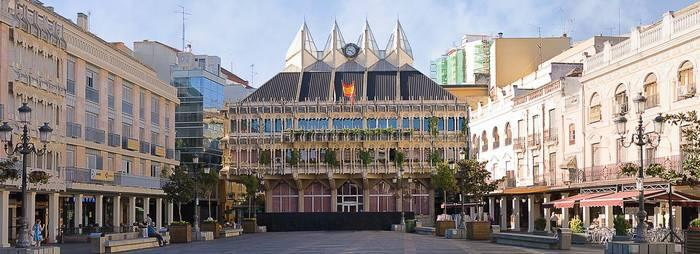
\includegraphics[width=1\linewidth,angle=0]{PlazaCR}
	\caption{Plaza de Ciudad Real}
	\label{fig:PlazaCR}
\end{figure}

% Dos subimagenes
\begin{figure}[htb]
	\centering
	\subfigure[Imagen de la fachada de la ESI]{
		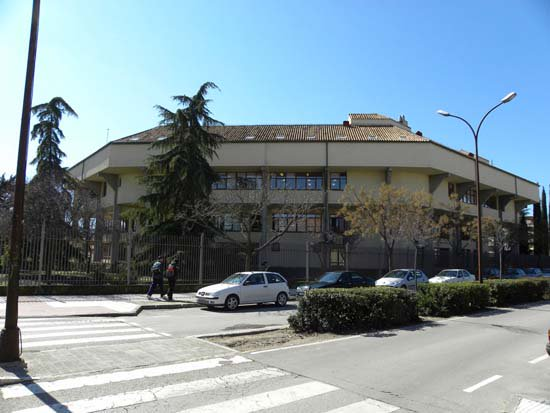
\includegraphics[width=7cm]{ESI2}
		\label{fig:ESI1}
	}
	\subfigure[Imagen de la ESI]{
		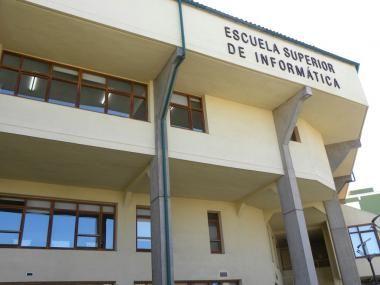
\includegraphics[width=7cm]{ESI1}
		\label{fig:ESI2}
	}
	\caption{Imágenes que muestran la ESI}
	\label{fig:ESI}
\end{figure}

Por último, para recrear la pulsación de un botón podemos usar: \tecla{Ctrl+C}


% Sección: Ejemplo de listados
\section{Ejemplo de listados}

El primer ejemplo consiste en un listado normal:
\begin{itemize}
	\item Item 1
	\item Item 2
	\item[\ding{108}] Se puede cambiar de icono usando ding. Consultar ChuLaTeX \cite{Salido2011}
	\item[*] Item 4
\end{itemize}

El segundo de un listado numerado:
\begin{enumerate}
	\item Item 1
	\item Item 2
	\item Item 3
	\item Item 4
\end{enumerate}

En este ejemplo vamos a mostrar el uso de un listado compacto:

\begin{compactitem}
	\item Item 1
	\item Item 2
	\item Item 3
	\item Item 4
\end{compactitem}


% Sección: Tablas
\section{Tablas}
Es posible introducir tablas en \LaTeX{}. Aquí se puede ver un pequeño ejemplo:

\begin{table}[htbp]
	\begin{center}
		\begin{tabular}{|l|l|}
			\hline
			Número de procesos & Tiempo (segundos) \\
			\hline \hline
			1 & 555,273043 \\ \hline
			4 & 278,392832 \\ \hline
			9 & 260,050554 \\ \hline
			16 & 251,819869 \\ \hline
			25 & 236,560818 \\ \hline
		\end{tabular}
		\caption{Resultado de la ejecución para matrices de orden N = 3600.}
		\label{tabla:Tiempos3600}
	\end{center}
\end{table}


% Sección: Referencias
\section{Añadir referencias}
Para el manejo de las referencias se recomienda la instalación de JabRef disponible en: \url{http://www.jabref.org/}. Mediante esta aplicación abrimos el archivo \emph{biblist.bib}. Mediante la aplicación introducimos las distintas referencias que queramos y a cada una le asignamos una bibtexkey que sea significativa para nosotros y no se repita.

Por último podemos citar libros o artículos mediante el comando cite. \cite{Kottwitz2011} \cite{Martin2017} \cite{Salido2011}. En este comando ponemos la bibtexkey que indica la referencia que queremos introducir.


% Sección: Mejoras y sugerencias
\section{Mejoras y sugerencias}
Puedes ayudar al desarrollo de esta plantilla aportando tus ideas, mejoras o sugerencias. Para ello puedes ponerte en contacto conmigo mediante la dirección de correo electrónico: \emph{joseangelmartinb@gmail.com}



%%%%%%%%%%%%%%%%%%%%%%%%%%%%%%%%%%%%%%%%%%%%%%%%%%%%%%%%%%%%%%%%%%%%%%%%%%%%%%%%
%%%%%%%%% 						BIBLIOGRAFIA 						   %%%%%%%%%
%%%%%%%%%%%%%%%%%%%%%%%%%%%%%%%%%%%%%%%%%%%%%%%%%%%%%%%%%%%%%%%%%%%%%%%%%%%%%%%%
\newpage
\bibliography{biblist}
\bibliographystyle{plain}
%\nocite{*} Permite citar todas las referencias en el archivo .bib

% Añadir la bibliografía al Índice de contenidos
\ifspanish
	\addcontentsline{toc}{section}{Referencias}
\else
	\addcontentsline{toc}{section}{References}
\fi



%%%%%%%%%%%%%%%%%%%%%%%%%%%%%%%%%%%%%%%%%%%%%%%%%%%%%%%%%%%%%%%%%%%%%%%%%%%%%%%%
%%%%%%%%% 					Atribución - ¡No Eliminar!				   %%%%%%%%%
%%%%%%%%%%%%%%%%%%%%%%%%%%%%%%%%%%%%%%%%%%%%%%%%%%%%%%%%%%%%%%%%%%%%%%%%%%%%%%%%
\null\vfill
\begin{center}
\ifspanish
	Este documento ha sido generado con \LaTeX{} utilizando la plantilla\\
	desarrollada por \textsc{José Ángel Martín Baos} y disponible en\\
	\url{https://github.com/JoseAngelMartinB/PlantillaTrabajosLaTeX}
\else
	This document was generated using \LaTeX{} and the template\\
	developed by \textsc{José Ángel Martín Baos} which is available in\\
	\url{https://github.com/JoseAngelMartinB/PlantillaTrabajosLaTeX}
\fi
\end{center}

\end{document}
